\documentclass[12pt,a4paper]{report}
\usepackage{amsmath}
\usepackage{amsfonts}
\usepackage{amssymb}
\usepackage{tikz}
\begin{document}
	\centering
	{\scshape\LARGE CS341 \par}
	{\scshape\Large Lecture 4\par}
	{\Large\itshape Yaro Gorban\par}
	{\large \today\par}
	\vspace{1.5cm}
	
	\textbf{Loop Analysis Slide 50:}
	\begin{itemize}
	\item each iteration of the while loop takes time $\Theta(1)$
	\item for a given value of i, how many iterations of the while loop are performed
	\end{itemize}
	 $\rightarrow \log i$ iterations \linebreak
	 $\rightarrow \sum^n_{i=1} \log i$ \linebreak
	 $\rightarrow$ via basic log rules $\log \prod^n_{i=1} i$ \linebreak
	 $\rightarrow \Theta (n!)$ \linebreak
	 $\rightarrow \Theta (n \log n)$ \linebreak
	\textbf{Recursion Tree Method:}
	\begin{itemize}
	\item Example: T(n) = 2T(n/2) + cn
	\item Create a tree with a root node of cn and 2 child nodes T(n/2)
	\end{itemize}
	\begin{center}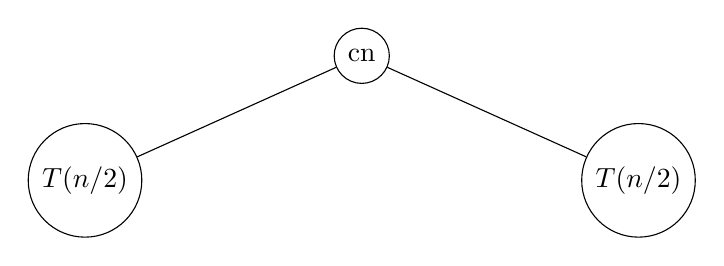
\begin{tikzpicture}[
  level distance=45 pt,
  every node/.style={circle,draw},
  level 1/.style={sibling distance=200 pt},
  level 2/.style={sibling distance=100 pt},
]
  \node {cn}
    child {node {$T(n/2)$}
    	child[missing]
    	child[missing]
    }
    child {node {$T(n/2)$}
    	child[missing]
    	child[missing]
    };
\end{tikzpicture}\end{center}
	\begin{itemize}
	\item This is still equal to T(n)
	\item Keep Splitting up until you see a pattern
	\item simplifies to dn + c$\log n$n
	\item So it is in $\Theta (n\log n)$
	\end{itemize}
\end{document}